\documentclass[a4paper,11pt]{article}

\usepackage{amsmath}
\usepackage[french]{babel}
\usepackage[T1]{fontenc}
\usepackage{graphicx}
\usepackage[utf8]{inputenc}
\usepackage{lmodern}
\usepackage{microtype}
\usepackage{natbib}
\usepackage{hyperref}

\title{<%= project_name %>}
\author{<%= user.first_name %> <%= user.last_name %>}
\date{<%= month %> <%= year %>}

\begin{document}

\maketitle

\section{Introduction}
L’ENSTA ParisTech propose à ses élèves une formation d’ingénieurs généralistes se donnant comme objectif de les rendre aptes à assurer la conception, la réalisation et la direction de systèmes industriels complexes, sous des contraintes économiques fortes et dans un environnement international.

\section{Latex}

\subsection{Apprendre le LaTex}

La meilleure ressource pour apprendre le LaTeX, c'est Babafou \citep{baudoin1994apprends}. Pour le pdf, c'est \href{http://www.babafou.eu.org/Apprends_LaTeX/Apprends_LaTeX.pdf}{là}.


\begin{figure}[h!]
\centering
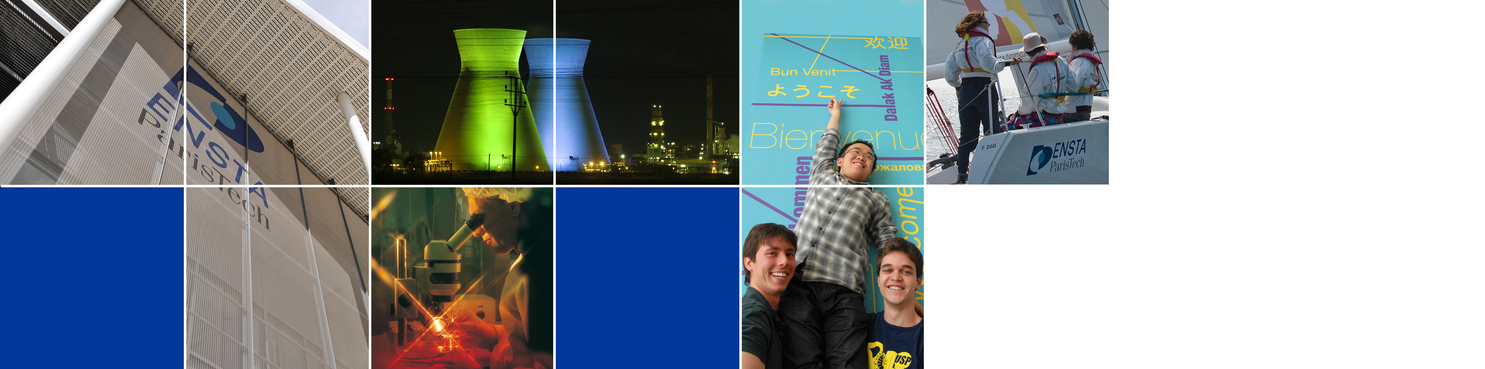
\includegraphics[width=\textwidth]{frise.jpg}
\caption{ENSTA Paristech}
\label{fig:ensta}
\end{figure}

\subsection{Pourquoi ces extensions}
Ces extensions sont celles conseillées par Babafou pour tout nouveau document !

\bibliographystyle{plain}
\bibliography{references}
\end{document}
